 
\begin{lrbox}{\methodologyoverviewbox}
\begin{minipage}{\linewidth}
\section{Methodology}
\label{sec:methodology}

Section~\ref{sec:proposed} introduced the seven modules of GRASP. Each module is described in the subsections below, in the order in which the data passes through the workflow, from a raw report to a final score. Figure~\ref{fig:architecture} uses the same titles as these subsections, so the diagram and the text can be read together. The first module collects the reports and stores them in a database. The stored data is then used to train the classifier, and three analysis branches draw on the same data to produce the outputs that the service delivers. The arrows in the figure mark only the main routes. Other database inputs and shared calculations are explained in the subsections. The Transparency Score combines four measures. These are the share of reporting items with a usable response, the share of text segments with an evidence marker, the share of text segments without a vagueness flag, and the number of Sustainable Development Goals (SDGs) linked through a fixed mapping. The third measure, Clarity, comes from the vagueness detector that is defined in the checks module and reused here. Principle probabilities and claim--figure flags are separate review outputs, so they do not enter the score.

\par\medskip
{\centering
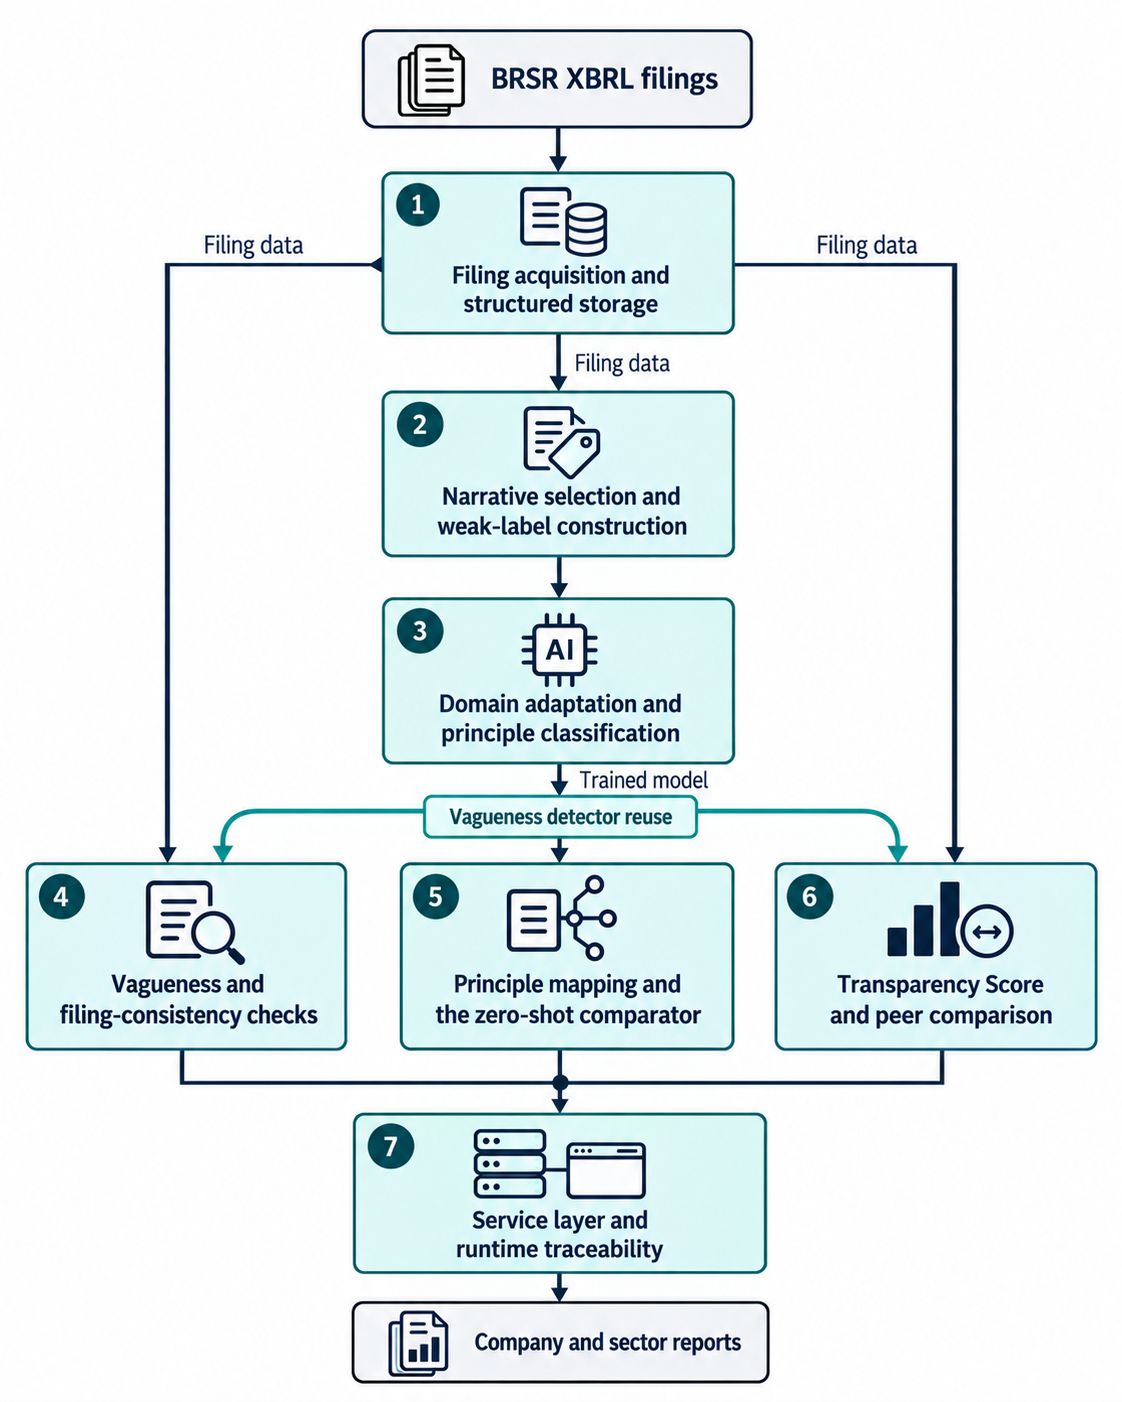
\includegraphics[width=0.98\linewidth,height=0.72\textheight,keepaspectratio]{figures/grasp_pipeline.png}
\captionof{figure}{GRASP workflow from BRSR filings to company and sector reports. Numbered modules correspond to the methodology subsections; arrows show the main data and model routes.}
\label{fig:architecture}
\par}

\end{minipage}
\end{lrbox}
\ifdim\dimexpr\ht\methodologyoverviewbox+\dp\methodologyoverviewbox\relax>\textheight
\PackageError{GRASP-layout}{Methodology overview exceeds one page}{Reduce the diagram height.}
\fi
\noindent\usebox{\methodologyoverviewbox}
\par\clearpage

Four counting units are used in a fixed way throughout the paper. A \emph{report} is the complete BRSR document filed by one company for one financial year. A \emph{text segment} is the selected portion of a report's text that is analysed, such as the written answer to one narrative question. A \emph{fact} is one reported value together with its concept, unit, and period. A \emph{dataset row} is one text segment stored with a label. These units have different counts. One company can file more than one report, and one report contains many text segments and facts. For example, the 6,201 test text segments come from 175 companies, so this number does not mean 6,201 reports or 6,201 companies.

Every subsection states five points in the same order: the input and where the input comes from, the processing steps, the model or rule used, the reference used for comparison, and the output with the meaning of the output.

\subsection{Report acquisition and structured storage}
\label{sec:ingestion}

\paragraph{Input.} The input is the set of BRSR reports submitted in eXtensible Business Reporting Language (XBRL), together with a company identifier for each report. In an XBRL file, each reported value is attached to a machine-readable label, so software can read the value without guessing what it means.

\paragraph{Processing.} A download log records which files were completed and which failed, so collection can resume after an interruption. The parser then reads the structured data directly. Three XBRL terms are used often. A \emph{concept} is the name of a reporting item, such as total water withdrawal. The \emph{context} tells which company and which period a value belongs to, and also holds any reporting categories. A \emph{unit} states how the value is measured, such as kilolitres \cite{xbrl2013}. With all three attached, a figure can always be compared with the correct company, period, and unit.

The parsed data is stored in three linked record types. A company record holds the Corporate Identity Number (CIN), the name, and the industry code. A report record holds the company link, the reporting dates, and the source location. A fact record holds the concept, the original value, the unit, the stated precision when available, the period, and the dimensions. Dimensions are reporting categories such as gender or employment type. Because of them, a workforce count is stored for each category and is not merged into one combined number. Values are stored as text and converted to numbers only when a calculation needs arithmetic. A company--year uniqueness rule allows one report per company and year, which prevents the same report from being loaded twice.

\paragraph{Model or rule.} This module needs no learning model. The parser follows the XBRL specification, and the uniqueness rule is a fixed rule in the database.

\paragraph{Comparison reference.} No comparison is made at this stage. The XBRL specification \cite{xbrl2013} defines the correct structure of the input.

\paragraph{Output.} The output is a searchable database of facts. A fact is stored together with four links: the source report, the concept, the period, and the unit. Later modules depend on these links. A text segment can be reviewed, a number can be compared, and a score can be calculated only because every fact can be traced back to the place where the value was filed.

\subsection{Text segment selection and weak-label construction}
\label{sec:labels}

\paragraph{Input.} The input is the stored text from the previous module. Candidate text segments come from concepts whose names contain \artifact{ExplanatoryTextBlock}. These concepts hold the narrative answers written by companies.

\paragraph{Processing.} The dataset builder first removes web links (URLs). A candidate is kept only if at least 15 words of useful content remain. Bare links, short fragments, and listed non-answers are removed. The company-scoring modules use different length rules, explained in Section~\ref{sec:score}. The text segments used for the classifier and the text segments used for scoring are therefore two different groups.

Each kept text segment then receives a \emph{weak label}. A weak label is a principle label assigned automatically from the structure of the report, instead of by a person reading the text. For example, a text segment filed under a question that belongs to Principle 6 receives the label P6. Three label sources are checked in a fixed order. First, an explicit \artifact{PrincipleAxis} tag in Section B of the report gives the label. Second, if that tag is missing, a concept-to-principle map for Section C gives the label. Third, a numbered \artifact{NotesPrincipleX} concept gives the label. The extension of the Section C map includes 29 AI-assisted assignments. When two maps overlap, the existing configured mapping takes priority. No independent expert has verified these 29 assignments.

Candidates are then grouped by company, concept, and cleaned text. Repeated entries with the same label become one dataset row. A group that carries several different labels is removed from the single-label dataset. Such groups include text covering several principles, and generic text reused under different questions.

\paragraph{Model or rule.} Fixed filtering and labelling rules are used. No model is trained in this module.

\paragraph{Comparison reference.} The weak labels become the reference answers for classifier training and testing. The CSV file records the label source of every dataset row for later analysis, but only the text of the segment enters the classifier.

\paragraph{Output.} The output is a dataset of 42,409 dataset rows, each with one principle label. The dataset is split by CIN. The training group contains 29,834 text segments from 814 companies. The validation group contains 6,374 text segments from 175 companies. The test group contains 6,201 text segments from 175 companies. No company appears in more than one group, and this split defines the main supervised evaluation. Exact wording shared by different companies is counted separately in the text-overlap check. Because the labels come from the structure of the report, agreement with the labels means agreement with the recorded assignment. Agreement is not an independent judgement of what the text means.

\subsection{Domain adaptation and principle classification}
\label{sec:classifier}

\paragraph{Input.} The input is the labelled dataset built in the previous module. Before training starts, the dataset is split by company into three groups. The training group holds 29,834 text segments from 814 companies and is used to fit the model. The validation group holds 6,374 text segments from 175 companies and is used to pick the best saved version. The test group holds 6,201 text segments from 175 companies and stays untouched until the final result is calculated.

\paragraph{Processing.} The classifier starts from \artifact{bert-base-uncased}, a BERT model that has already read a very large body of general English text \cite{devlin2019}. Training then runs in two steps. The first step is \emph{masked language modelling}, which adapts the model to sustainability language. A few word pieces in a text segment are hidden, and the model has to guess each hidden piece from the surrounding words. For example, in the sentence \emph{the plant reduced [hidden] withdrawal by 5\%}, the model should recover the word \emph{water}. The second step adds a nine-output classification layer on top of BERT. Labelled training then teaches the model to choose among the nine principles \cite{gururangan2020}.

Several settings control the training. The classifier accepts at most 512 \emph{tokens}, which are word pieces produced by the tokenizer. Dynamic padding adds only the padding needed inside each batch. Training processes four text segments at a time and combines the gradients of four such groups before each update, so every update uses 16 text segments. Fine-tuning runs for five epochs, and an \emph{epoch} is one full pass through the training group. In each update, the learning rate of $2\times10^{-5}$ sets how far the parameters move. The rate does not start at that value. It rises gradually over the first 300 steps (warmup) and then falls along a smooth curve (cosine decay). A weight decay of 0.01 keeps the parameters from growing too large.

The loss function is cross-entropy. When the model gives a low probability to the correct label, the penalty is high. Principles with few training text segments could be ignored by the model, so each class is given a weight equal to the square root of the inverse training frequency. A rare principle therefore counts for more, and the square root stops this boost from becoming too large. Training also depends on a random seed. Fixing the seed makes a run repeatable, and five seeds (42, 1, 7, 99, and 2024) were compared using validation macro-F1. Seed 99 gave the best result, and its checkpoint 7,460 is the audited final classifier. A \emph{checkpoint} is a saved copy of the model parameters at one point in training.

The saved seed-99 file used older names (\artifact{gamma} and \artifact{beta}) for 50 LayerNorm parameters. LayerNorm is a layer that keeps values in a stable range. Current software expects the names \artifact{weight} and \artifact{bias}. Checkpoint recovery renames these 50 parameters, requires every parameter to load, and confirms that the model is identical after saving and reloading. No further training takes place during recovery, and all test results come from the recovered model.

\paragraph{Model or rule.} For a text segment $x$, the model produces nine raw scores, called \emph{logits}, one for each principle. Softmax converts the logits $z_1,\dots,z_9$ into probabilities:
\begin{equation}
p_k(x)=\frac{\exp(z_k)}{\sum_{j=1}^{9}\exp(z_j)}.
\label{eq:softmax}
\end{equation}
Here, $p_k(x)$ is the probability that text segment $x$ belongs to principle $k$, and the nine probabilities add up to 1. The largest probability gives the Top-1 prediction, and the two largest probabilities give the Top-2 candidate list. MPNet is not used for classification. MPNet supplies sentence similarity for the checks module and for the zero-shot comparison.

\paragraph{Comparison reference.} The validation weak labels select the checkpoint, and the test weak labels give the final agreement score. Earlier ClimateBERT and ensemble runs belong to the experiment history and are not part of the final evaluation.

\paragraph{Output.} The output is a set of nine principle probabilities for each text segment, together with the Top-1 and Top-2 predictions. One limit applies to the company separation. The earlier masked-language-model builder read text across the whole company database, and the adaptation membership of the selected checkpoint has not been verified. The company-separation checks therefore apply to labelled fine-tuning only.

\subsection{Vagueness detection and report-consistency checks}
\label{sec:detector}

This module produces two kinds of review output. The first is the \emph{language branch}, a vagueness detector. A text segment is flagged when its wording is unclear and no concrete evidence supports the wording. The same detector is reused in Section~\ref{sec:score} to calculate Clarity. The second is the \emph{numerical branch}, which produces claim--figure, assurance-gap, and omission records. These records are separate review outputs and do not enter the Transparency Score. Section~\ref{sec:evaluation} reports the evaluation data for each measured component.

\subsubsection{Hedging words and evidence markers}

\paragraph{Input.} The input is the text segments taken from the stored text-block facts.

\paragraph{Processing.} The detector looks for two opposite things in each text segment: hedging and evidence. Hedging is found with a word list that covers four kinds of wording. These are promises, conditional commitments, unclear time expressions, and progress claims that give no measure. Take the sentence \emph{the company aims to improve water use in the coming years}. It contains a promise and an unclear time, and no measure is given. Evidence is found with patterns for percentages, currency amounts, physical quantities, workforce or incident counts, reporting years, named standards, and selected formal governance systems. In the code, a match is stored as the marker \artifact{has_kpi}. A sentence such as \emph{Emissions fell by 12\% in FY2025--26} carries this marker, because the sentence gives a percentage and a reporting year.

\paragraph{Model or rule.} A text segment is flagged when the text segment contains hedging and no evidence marker. If the text segment is longer than 80 words, the hedging density must also reach 0.005. Hedging density is the number of matches divided by the number of words. A separate rule flags bare URLs and listed website redirects. The final pattern set requires digits in currency matches, includes MW and GW units and statutory terms, and handles URL redirects explicitly.

\paragraph{Comparison reference.} The patterns are compared with the text of each text segment. No external reference is used at this step.

\paragraph{Output.} The output is three signals for each text segment: a hedging flag, an evidence-marker status, and a URL flag. The evidence-marker status is also used for Specificity in Section~\ref{sec:score}.

\subsubsection{Comparing sentence meanings}

\paragraph{Input.} The input is the same text segments, split into sentences.

\paragraph{Processing.} The \artifact{all-mpnet-base-v2} encoder turns each sentence into a \emph{vector}, which is a list of numbers that represents the meaning of the sentence \cite{reimers2019,song2020}. Cosine similarity measures how close two vectors are. Every sentence vector is compared with two fixed reference sets, one of vague statements and one of specific statements. Let $v_j$ be the largest similarity between sentence $j$ and any vague reference. Let $q_j$ be the largest similarity between sentence $j$ and any specific reference. The sentence with the largest value of $q_j-v_j$ is selected as the most specific sentence of the text segment, and the decision is based on this sentence.

\paragraph{Model or rule.} Without an evidence marker, a text segment is flagged when $v_j\geq0.42$ and $v_j>q_j$. With an evidence marker, the rule is stricter, and a text segment is flagged only when $v_j\geq0.58$ and $v_j-q_j\geq0.15$. A URL-redirect match takes priority over both rules. The final detector flags a text segment when either the word-list rule or the similarity rule applies.

\paragraph{Comparison reference.} The freeze file records the detector version and all thresholds before the audited run, and the settings stay fixed during evaluation. Batches 1 and 2 form the 80-example development group.

\paragraph{Output.} The output is one vagueness flag for each text segment. A flag means that the wording is a candidate for review. A flag does not prove that the company misled the reader.

\subsubsection{Claim--figure, assurance, and omission checks}

\paragraph{Input.} The input is the sentences of the text segments, together with the facts of the same report. The previous-period and current-period values of each concept come from the fact records.

\paragraph{Processing.} The claim--figure check covers four topics: emissions, water, waste, and non-renewable energy. A sentence qualifies only when the sentence contains both improvement wording and a phrase linked to the measure. If the filed value for that measure increased, a review record is created. For illustration, suppose a sentence reports a reduction in Scope 1 emissions, while the filed Scope 1 value rises from 4,142.84 to 5,177.03 tCO\textsubscript{2}e. The check then creates a record. Matching inside one sentence avoids accidental links, such as comparing a Scope 2 reduction claim with a Scope 1 increase. The record keeps the sentence, the concept, the previous and current values, and the assurance information.

The assurance-gap rule links a domain-specific fact with the assurance information reported for the same domain. The omission rule finds a concept that has a value in the previous period and no matching value in the current period.

\paragraph{Model or rule.} All three checks are fixed rules, and no learning model is used.

\paragraph{Comparison reference.} A check never judges a text segment on its own. The sentence is set against the filed values of the same report. For example, a sentence about Scope 1 emissions is compared with the Scope 1 figures of the two years. A match of this kind is only the start of the review. The next step is to open the linked report context and look for five things. These are what the measure actually covers, whether the figure is a total or a per-output quantity, the unit, the period, and the business boundary.

\paragraph{Output.} Each check produces a rule-generated review record. Each record points the analyst to a place worth reading and is not a verdict. A record can be wrong, so the rules behind the records need to be known. The assurance-gap rule finds a fact from the right domain, but period, unit, and dimension are not fully restricted when the fact is chosen. The same rule reads a text value of zero as missing, and the omission rule skips some previous entries whose value is zero. Completeness is different. A structured zero is a valid response there, so the zero is counted. Before trusting a record, the analyst should therefore look at the original values and the reporting categories. The accuracy results in Section~\ref{sec:evaluation} cover the language branch only, and the numerical records are not part of the Transparency Score.

\subsection{Principle mapping and the zero-shot comparator}
\label{sec:mapping}

\paragraph{Input.} The input is the text segments of a report, each with a recorded principle assignment, and the recovered classifier from Section~\ref{sec:classifier}.

\paragraph{Processing.} The classifier produces nine probabilities for every text segment using Equation~\eqref{eq:softmax}. Reusing the trained classifier for this task is called \emph{supervised transfer} in the evaluation. For all text segments filed under principle $k$, the service averages $p_k(x)$ and also keeps the lowest-scoring text segment for inspection. The company summary then averages the available principle means.

\paragraph{Model or rule.} The mean for principle $k$ is
\begin{equation}
\bar{p}_k=\frac{1}{N_k}\sum_{x\in X_k}p_k(x),
\label{eq:mapmean}
\end{equation}
where $X_k$ is the set of text segments filed under principle $k$, and $N_k=|X_k|$ is the number of text segments in the set. The company summary is the average of $\bar{p}_k$ over all principles that have at least one text segment. This value describes how strongly the model supports the recorded principle assignment.

A \emph{zero-shot} method serves as the comparator. Zero-shot means that the ranking method is not fitted to the principle-labelled training set. MPNet vectors are used for the same test text segments. Each principle has an expanded definition and a fixed set of example text segments, called \emph{anchors}. The ranking score for principle $k$ is
\begin{equation}
z_k(x)=0.50\,d_k(x)+0.50\left[0.70\max_a s_{ka}(x)+0.30\,\operatorname{mean}_a s_{ka}(x)\right].
\label{eq:hybrid}
\end{equation}
In Equation~\eqref{eq:hybrid}, $d_k(x)$ is the similarity between text segment $x$ and the definition of principle $k$, and $s_{ka}(x)$ is the similarity between $x$ and anchor $a$ of principle $k$. The score gives equal weight to the definition and to the anchors. Inside the anchor part, 70\% of the weight goes to the best-matching anchor and 30\% to the average of all anchors.

\paragraph{Comparison reference.} Both methods rank the nine principles for the same 6,201 test text segments, and both are compared with the weak labels defined in Section~\ref{sec:labels}. The supervised classifier has seen training labels, and the zero-shot method has not. The difference therefore combines the effect of the model representation and the effect of labelled training.

\paragraph{Output.} The output has two parts. The first is the company-level principle summary used by the service. The second is the supervised-versus-zero-shot comparison reported in Section~\ref{sec:evaluation}.

\subsection{Transparency Score and peer comparison}
\label{sec:score}

\paragraph{Input.} The input is the facts and the scoring text segments of one report, the fixed concept list of the database, the vagueness detector from Section~\ref{sec:detector}, and the recorded industry code. Scoring text segments follow their own length rules, described below, and are not the same group as the classifier text segments in Section~\ref{sec:labels}.

\paragraph{Processing and formula.} The Transparency Score combines four percentages, each on a 0--100 scale:
\begin{equation}
TS_f=0.40\,C_f+0.30\,Sp_f+0.20\,Cl_f+0.10\,G_f.
\label{eq:ts}
\end{equation}
Here, $f$ is one report, $C$ is Completeness, $Sp$ is Specificity, $Cl$ is Clarity, and $G$ is SDG breadth. The weights 0.40/0.30/0.20/0.10 are fixed in the implementation. Each component and the final sum are rounded to two decimal places. The four components are explained below.

\subsubsection{Completeness: which reporting items have a usable response?}

Completeness works like a checklist. The saved database holds 1,057 distinct concept names, covering structured and narrative items alike, and this checklist is written $U$. For a report $f$, the concepts that received at least one accepted response form the set $A_f$. Completeness is the percentage of the checklist that the report answers:
\begin{equation}
C_f=100\,\frac{|A_f|}{|U|}.
\label{eq:complete}
\end{equation}
Every report is divided by the same 1,057, even when some items belong to other sectors, so all companies stay on one scale. A concept is counted once, however many dimensions carry a value for the concept. The Triveni Turbine report in Section~\ref{sec:case} shows the calculation: 613 accepted concepts out of 1,057 give $C=57.99\%$.

Not every answer is accepted. Blank answers are rejected, and so are placeholders such as \emph{NA} and \emph{not applicable}. A structured zero is accepted, since zero can be a true reported value. Narrative text blocks are checked more strictly. Placeholders and a lone zero are rejected. Text longer than 30 characters must contain at least ten words, whereas a shorter value is accepted when no placeholder matches. Address fields follow a separate rule.

\subsubsection{Specificity: how often does a text segment contain an evidence marker?}

Scoring uses text-block facts with at least 30 characters. Duplicate concept--text pairs are removed after extra spaces are trimmed. The same wording under different concepts can still count as several text segments. Let $N_f$ be the number of retained text segments in report $f$. Let $K_f$ be the number of those text segments with at least one evidence marker from Section~\ref{sec:detector}. Specificity is
\begin{equation}
Sp_f=100\,\frac{K_f}{N_f}.
\label{eq:specificity}
\end{equation}
For example, 20 marked text segments out of 40 retained text segments give $Sp=50\%$. A text segment with five numbers counts once, and so does a text segment with one recognised standard. The denominator is the number of text segments, not the number of numbers.

\subsubsection{Clarity: how much text avoids a vagueness flag?}

Clarity does not need a new detector. The vagueness detector from Section~\ref{sec:detector} is run again on the scoring text segments, with the same word lists, thresholds, and URL rule. For a report $f$, let $V_f$ be the number of retained scoring text segments that the detector flags, and let $N_f$ be the total number of retained scoring text segments, the same count used for Specificity. Clarity is the percentage of text segments that are left without a flag:
\begin{equation}
Cl_f=100\left(1-\frac{V_f}{N_f}\right).
\label{eq:clarity}
\end{equation}
The Triveni Turbine report in Section~\ref{sec:case} shows the calculation. One of its 52 retained text segments is flagged, so $Cl=100\times(1-1/52)=98.08\%$. If a report has no scoring text segments, the code returns zero for both Specificity and Clarity.

In Equation~\eqref{eq:ts}, Clarity has a weight of 20\%. A high value tells the reader only that vague wording is rare. The text segments may still contain no concrete evidence, and that point is measured separately by Specificity. The claim--figure, assurance-gap, and omission records from Section~\ref{sec:detector} are not part of Equation~\eqref{eq:ts}.

\subsubsection{SDG breadth: how many goals are linked to marked text segments?}

SDG breadth connects the nine BRSR principles to the 17 United Nations Sustainable Development Goals (SDGs) \cite{un2015}. A principle counts only when it has proof of concrete disclosure. This means that an explicitly tagged narrative of the principle has at least 20 characters and contains an evidence marker. Each principle is tied to goal numbers through a fixed map. P1 maps to goal 16, and P2 and P9 both map to goals 9 and 12. P3 maps to goals 3, 5, and 8, while P4 maps to goals 10 and 17. P5 maps to goals 8, 10, and 16. P6 has the widest link, with goals 6, 7, 12, 13, and 15. P7 maps to goals 16 and 17, and P8 maps to goals 1, 8, 10, and 11. Let $D_f$ be the set of principles that count in report $f$, and let $M(k)$ be the goals mapped to principle $k$. SDG breadth is the percentage of the 17 goals reached by these principles:
\begin{equation}
G_f=100\,\frac{\left|\bigcup_{k\in D_f}M(k)\right|}{17}.
\label{eq:sdg}
\end{equation}
Goals are counted by their number and not by how often they appear, so a goal reached through two principles is counted once. For example, if only P1 and P7 qualify, the goals reached are 16 and 17, and $G=100\times2/17=11.76\%$. The map touches only 14 of the 17 goals, so the highest possible value is 82.35\%. The calculation follows the fixed map and does not check the 169 individual SDG targets. Saved exports call this component \emph{SDG Alignment}, but the calculation measures how many goals are reached, which is why the paper uses the name SDG breadth. When the same concept--text pair appears under more than one principle, only one principle is kept, chosen by database record order.

\subsubsection{Sector grouping and percentiles}

A score means more when it is read against companies of the same kind, so each company is placed in a sector. The placement uses the recorded industry code and a local mapping. The financial analysis uses the saved group \emph{Financial Services (excl. Insurance)}, while insurance and auxiliary financial services remain separate groups. For company $c$ in sector $S$, the percentile is
\begin{equation}
P_c=100\,\frac{\#\{j\in S:TS_j<TS_c\}}{|S|}.
\label{eq:percentile}
\end{equation}
In this formula, $|S|$ is the number of companies in the sector. The numerator counts the companies whose score is strictly lower than the score of company $c$. Suppose a sector has 20 companies and 15 of them score below company $c$. Then $P_c=100\times15/20=75$. Companies with tied scores receive the same percentile, so the highest percentile in a sector need not reach 100. The main sector comparison keeps only groups with at least five companies, because a percentile in a very small group says little. Sector means, medians, ranges, and standard deviations describe the scores inside each group.

\paragraph{Comparison reference.} A company score is compared with the sector peers and with the sector summary statistics. Section~\ref{sec:evaluation} also compares the score with 20 historical human ratings.

\paragraph{Output.} Each company ends with one Transparency Score, four component percentages, and a sector percentile. Together, these values show how much of the reporting is covered, how often evidence markers appear, how much wording is vague, and how many SDGs are reached. They help an analyst decide where to start a review. They do not prove greenwashing.

\subsection{Service layer and runtime traceability}
\label{sec:api}

\paragraph{Input.} The input is the stored database, the classifier outputs, the review records, and the saved scores from the previous modules.

\paragraph{Processing.} An application programming interface (API) provides company search, report analysis, score breakdowns, peer comparisons, and principle mapping. The principle-mapping endpoint returns the method name and the model path, so an operator can identify which classifier produced the result. The verified route reports \artifact{recovered_seed99_supervised_classifier} and uses the recovered checkpoint from Section~\ref{sec:classifier}. If this classifier is unavailable, the endpoint returns an error, so a different method is never shown under the same label.

\paragraph{Model or rule.} The service applies no new model or formula. Model-loading status, text segment probabilities, and peer comparisons are returned in separate response fields.

\paragraph{Comparison reference.} The audit checks the returned method name and checkpoint path against the recovered seed-99 classifier.

\paragraph{Output.} The audit records one successful request for one company. The returned mean probability summarises the report of that company. The request confirms that the correct model was loaded, but the request does not evaluate model quality.